%%%%%%%%%%%%%%%%%%%%%%%%%%%%%%%%%%%%%%%%%%%%%%%%%%%%%%%%%%%%%%%
% IMPORTANTE: Compilar con XeLaTeX
% Proyecto aplicado - Análisis de Regresión EYP2307
%%%%%%%%%%%%%%%%%%%%%%%%%%%%%%%%%%%%%%%%%%%%%%%%%%%%%%%%%%%%%%%

\documentclass{style}

%%%%%%%%%%%%%%%%% CONFIGURACIONES GENERALES %%%%%%%%%%%%%%%%%
\graphicspath{{./figures/}{./img/}}

\renewcommand{\contentsname}{Índice de contenido}
\renewcommand{\listfigurename}{Índice de figuras}
\renewcommand{\listtablename}{Índice de tablas}
\renewcommand{\tablename}{Tabla}
\renewcommand{\figurename}{Figura}
\addto\captionsspanish{\renewcommand{\tablename}{Tabla}\renewcommand{\figurename}{Figura}}

\newcommand{\var}[1]{\texttt{#1}}
\setstretch{1.03}
\setlength{\parskip}{0.25em}
\emergencystretch=2em
\captionsetup[figure]{font=footnotesize,skip=10pt}
\captionsetup[table]{font=footnotesize,skip=5pt}
\newcommand{\reporttablesize}{\footnotesize}

%%%%%%%%%%%%%%%%% DOCUMENTO %%%%%%%%%%%%%%%%%
\begin{document}

% Se deja el encabezado UC dentro del cuerpo del documento para asegurar que el logo se vea.
\pagestyle{plain}

%%%%%%%%%%%%%%%%% BLOQUE SUPERIOR UC %%%%%%%%%%%%%%%%%
\noindent
\begin{minipage}{0.14\textwidth}
    
\includegraphics[width=1.8cm]{img/logo-uc-3.pdf}
\end{minipage}
\hfill
\begin{minipage}{0.82\textwidth}
    {\small
    \textsc{Pontificia Universidad Católica de Chile}\\
    \textsc{Facultad de Matemáticas}\\
    \textsc{Departamento de Estadística}\\
    \textsc{EYP2307 -- Análisis de Regresión}
    }
\end{minipage}

\vspace{0.35cm}
\hrule
\vspace{0.35cm}

\begin{center}
    {\Large \textbf{Avance Proyecto de Regresión: Magnitud de eventos sísmicos USGS 2024}}\\[0.2cm]
    {\normalsize Primer Semestre 2026}
\end{center}

\vspace{0.2cm}

%%%%%%%%%%%%%%%%% 1. PREGUNTA Y CONTEXTO %%%%%%%%%%%%%%%%%
\section{Pregunta y contexto}

La pregunta de investigación es: \textbf{¿Cómo se asocia la magnitud de los eventos sísmicos registrados por USGS durante 2024 con su profundidad, localización geográfica y características técnicas del registro?}

La variable respuesta es la magnitud reportada del evento, \var{mag}. El enfoque del proyecto es descriptivo-explicativo: se busca estimar asociaciones promedio dentro del catálogo observado, no predecir terremotos futuros ni construir un sistema operacional de alerta. La pregunta es abordable con regresión lineal porque la respuesta es numérica y los predictores candidatos incluyen variables continuas, transformaciones y variables categóricas representables mediante indicadores.

La interpretación de fondo se centra en cómo varía la magnitud reportada según profundidad, posición geográfica y características técnicas del registro sísmico. Una limitación central es que la muestra está truncada a eventos con magnitud al menos 4, por lo que las conclusiones no se extrapolan a sismos menores ni al proceso sísmico completo.

%%%%%%%%%%%%%%%%% 2. FUENTE, DATOS Y ÉTICA %%%%%%%%%%%%%%%%%
\section{Fuente, datos y ética}

La fuente es el \textit{USGS Earthquake Catalog}, catálogo oficial y público del \textit{U.S. Geological Survey}. La unidad de observación es un evento sísmico registrado durante 2024 con \var{mag} mayor o igual a 4. Después de la limpieza inicial se mantienen 14.176 eventos. Los predictores candidatos son \var{depth}, \var{latitude}, \var{longitude}, \var{nst}, \var{gap}, \var{dmin}, \var{rms}, \var{magType}, \var{net}, \var{month}, \var{hour} y una región aproximada derivada desde \var{place}.

La selección de predictores combina tres criterios. Primero, interpretabilidad de fondo: profundidad y coordenadas describen rasgos geofísicos básicos del evento. Segundo, calidad y cobertura del registro: \var{nst}, \var{gap}, \var{dmin} y \var{rms} resumen cuántas estaciones participan, cómo rodean al epicentro, qué tan cerca está la estación más próxima y qué tan bien ajusta la solución reportada. Tercero, codificación del catálogo: \var{magType} y \var{net} permiten controlar diferencias promedio por escala de magnitud y red reportante. Las correlaciones y gráficos bivariados apoyan la selección al detectar asociación y colinealidad, pero no son una regla automática ni implican causalidad.

{\reporttablesize
\begin{tabularx}{\textwidth}{@{}p{0.27\textwidth}X@{}}
\toprule
Campo & Descripción \\
\midrule
Fuente & U.S. Geological Survey, Earthquake Catalog API. \\
Contexto & Eventos sísmicos registrados durante 2024 con magnitud al menos 4. \\
Unidad de observación & Evento sísmico registrado en el catálogo. \\
Variable dependiente numérica & Magnitud del evento (mag). \\
Predictores candidatos & depth, latitude, longitude, nst, gap, dmin, rms, magType, net, month, hour y region\_from\_place. \\
Tamaño muestral & 14,176 eventos después de la limpieza inicial. \\
Datos faltantes & dmin (0.37\%); gap (0.37\%); nst (0.36\%); rms (0.01\%) \\
Dificultades del análisis & Truncamiento por mag >= 4; asimetría o concentración de magnitudes; valores atípicos; faltantes en variables técnicas; posible colinealidad; dependencia espacial; categóricas con muchas categorías; variables técnicas no necesariamente causales. \\
\bottomrule
\end{tabularx}

}

Los datos no contienen información personal y el riesgo ético directo es bajo. Aun así, el uso responsable exige evitar conclusiones de seguridad pública, alertas o lenguaje de predicción operacional. Las variables técnicas pueden asociarse con la magnitud reportada, pero no se interpretan como causas físicas directas.

\begin{table}[H]
\centering
\caption{Significado y justificación de variables usadas}
\reporttablesize
\begin{tabularx}{\textwidth}{@{}p{0.24\textwidth}p{0.35\textwidth}X@{}}
\toprule
Variable & Qué significa & Por qué se usa \\
\midrule
\var{mag} & Magnitud reportada por USGS; es la respuesta numérica. & Permite estimar diferencias promedio dentro de eventos con \var{mag} $\geq$ 4. \\
\var{depth}, \var{log\_depth\_plus\_1} & Profundidad estimada del evento y su transformación logarítmica. & Profundidad es interpretable y \var{log\_depth\_plus\_1} reduce asimetría y peso de valores extremos. \\
\var{latitude}, \var{longitude} & Coordenadas del epicentro. & Controlan concentración espacial observada en el mapa y diferencias geográficas promedio. \\
\var{nst} & Número de estaciones usadas en la solución. & Resume cobertura del registro; más estaciones pueden asociarse con eventos mejor observados. \\
\var{gap} & Brecha azimutal de estaciones alrededor del epicentro. & Mide geometría de cobertura; valores altos sugieren menor cobertura angular. \\
\var{dmin} & Distancia mínima a una estación reportante. & Resume proximidad del registro y disponibilidad de información cercana. \\
\var{rms} & Error cuadrático medio del ajuste del evento. & Resume ajuste técnico de la localización; se interpreta como característica del registro. \\
\var{magType\_grouped}, \var{net\_grouped} & Tipo de magnitud y red reportante, agrupados. & Controlan diferencias de codificación y reporte sin crear categorías con muy pocos casos. \\
\var{month}, \var{hour}, \var{region\_grouped} & Variables temporales y región derivada desde \var{place}. & Apoyan el EDA y revisan composición temporal/geográfica del catálogo. \\
\bottomrule
\end{tabularx}
\end{table}

%%%%%%%%%%%%%%%%% 3. LIMPIEZA INICIAL Y EDA %%%%%%%%%%%%%%%%%
\section{Limpieza inicial y EDA}

La limpieza inicial convierte \var{time} a fecha-hora UTC, fuerza variables numéricas con \var{errors="coerce"}, deriva \var{month}, \var{hour}, \var{weekday}, crea \var{log\_depth\_plus\_1} como una transformación logarítmica de \var{depth}, y extrae \var{region\_from\_place} desde el texto de localización. Se revisan duplicados por \var{id}, rangos plausibles y faltantes. No se eliminan automáticamente valores atípicos de magnitud o profundidad; para los modelos preliminares se usa eliminación por lista solo en las variables de cada fórmula.

{\reporttablesize
\begin{tabular}{ll}
\toprule
revisión & resultado \\
\midrule
Duplicados por id & 0 registros involucrados (0 ids duplicados). \\
Rango observado de mag & 4.0 a 7.5 \\
Rango observado de depth & -0.070 a 671.043 \\
Rango observado de latitude & -65.301 a 86.605 \\
Rango observado de longitude & -179.999 a 179.998 \\
Profundidades negativas & 1 evento; se reporta y no se elimina automáticamente. \\
Faltantes principales & dmin: 52 (0.37\%); gap: 52 (0.37\%); nst: 51 (0.36\%); rms: 1 (0.01\%) \\
\bottomrule
\end{tabular}

}

La revisión confirma que no hay duplicados por \var{id}. Los faltantes principales se concentran en \var{dmin}, \var{gap}, \var{nst} y \var{rms}, mientras que \var{mag}, \var{depth}, \var{latitude} y \var{longitude} no presentan faltantes en la base procesada. Las variables categóricas \var{magType}, \var{net} y \var{region\_from\_place} se agrupan conservando niveles frecuentes y reuniendo categorías escasas como \textit{Other}; esto reduce indicadores con pocas observaciones y mejora la estabilidad de los modelos lineales preliminares.

\begin{figure}[H]
\centering
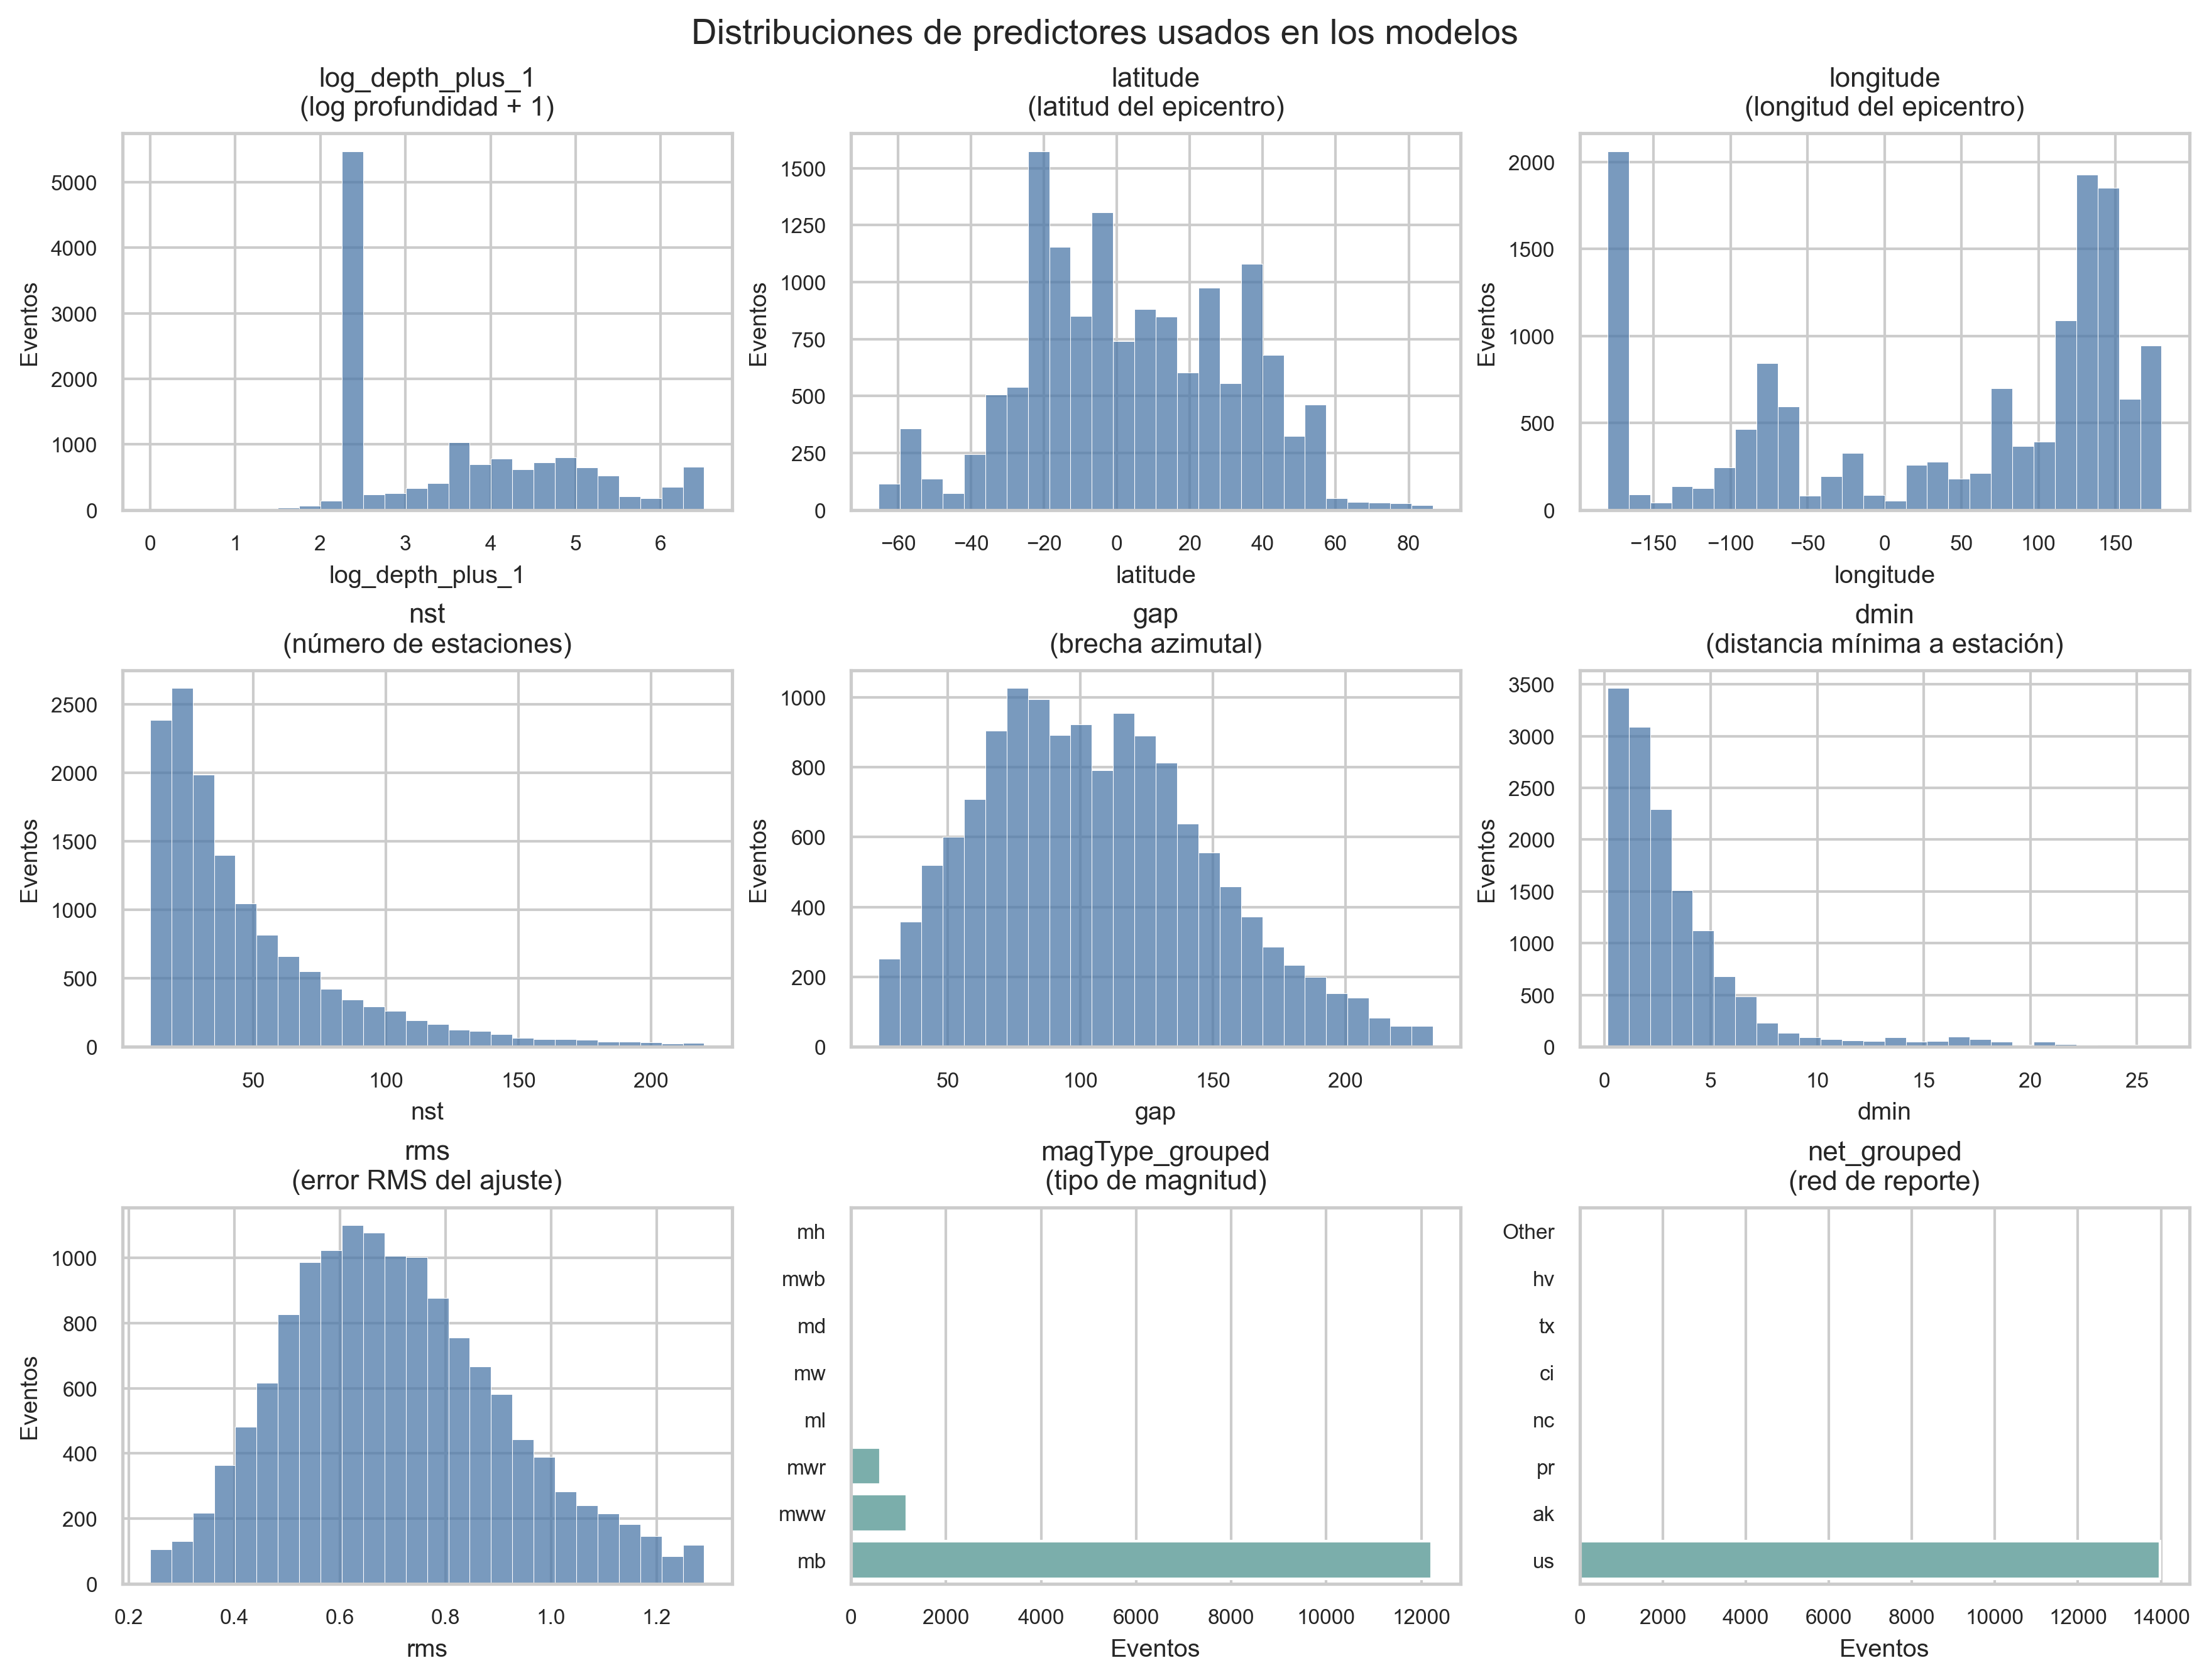
\includegraphics[width=0.88\textwidth]{fig_covariate_distributions.png}
\vspace{0.12cm}
\caption{Distribuciones de predictores usados en los modelos principales. Cada panel indica el nombre de la variable y su significado entre paréntesis. Las variables numéricas se muestran con histogramas y las categóricas agrupadas con barras; en variables muy asimétricas se usa el rango p1--p99 solo para visualización, sin eliminar observaciones de la base analítica.}
\end{figure}

\begin{figure}[H]
\centering
\begin{subfigure}{0.48\textwidth}
    \centering
    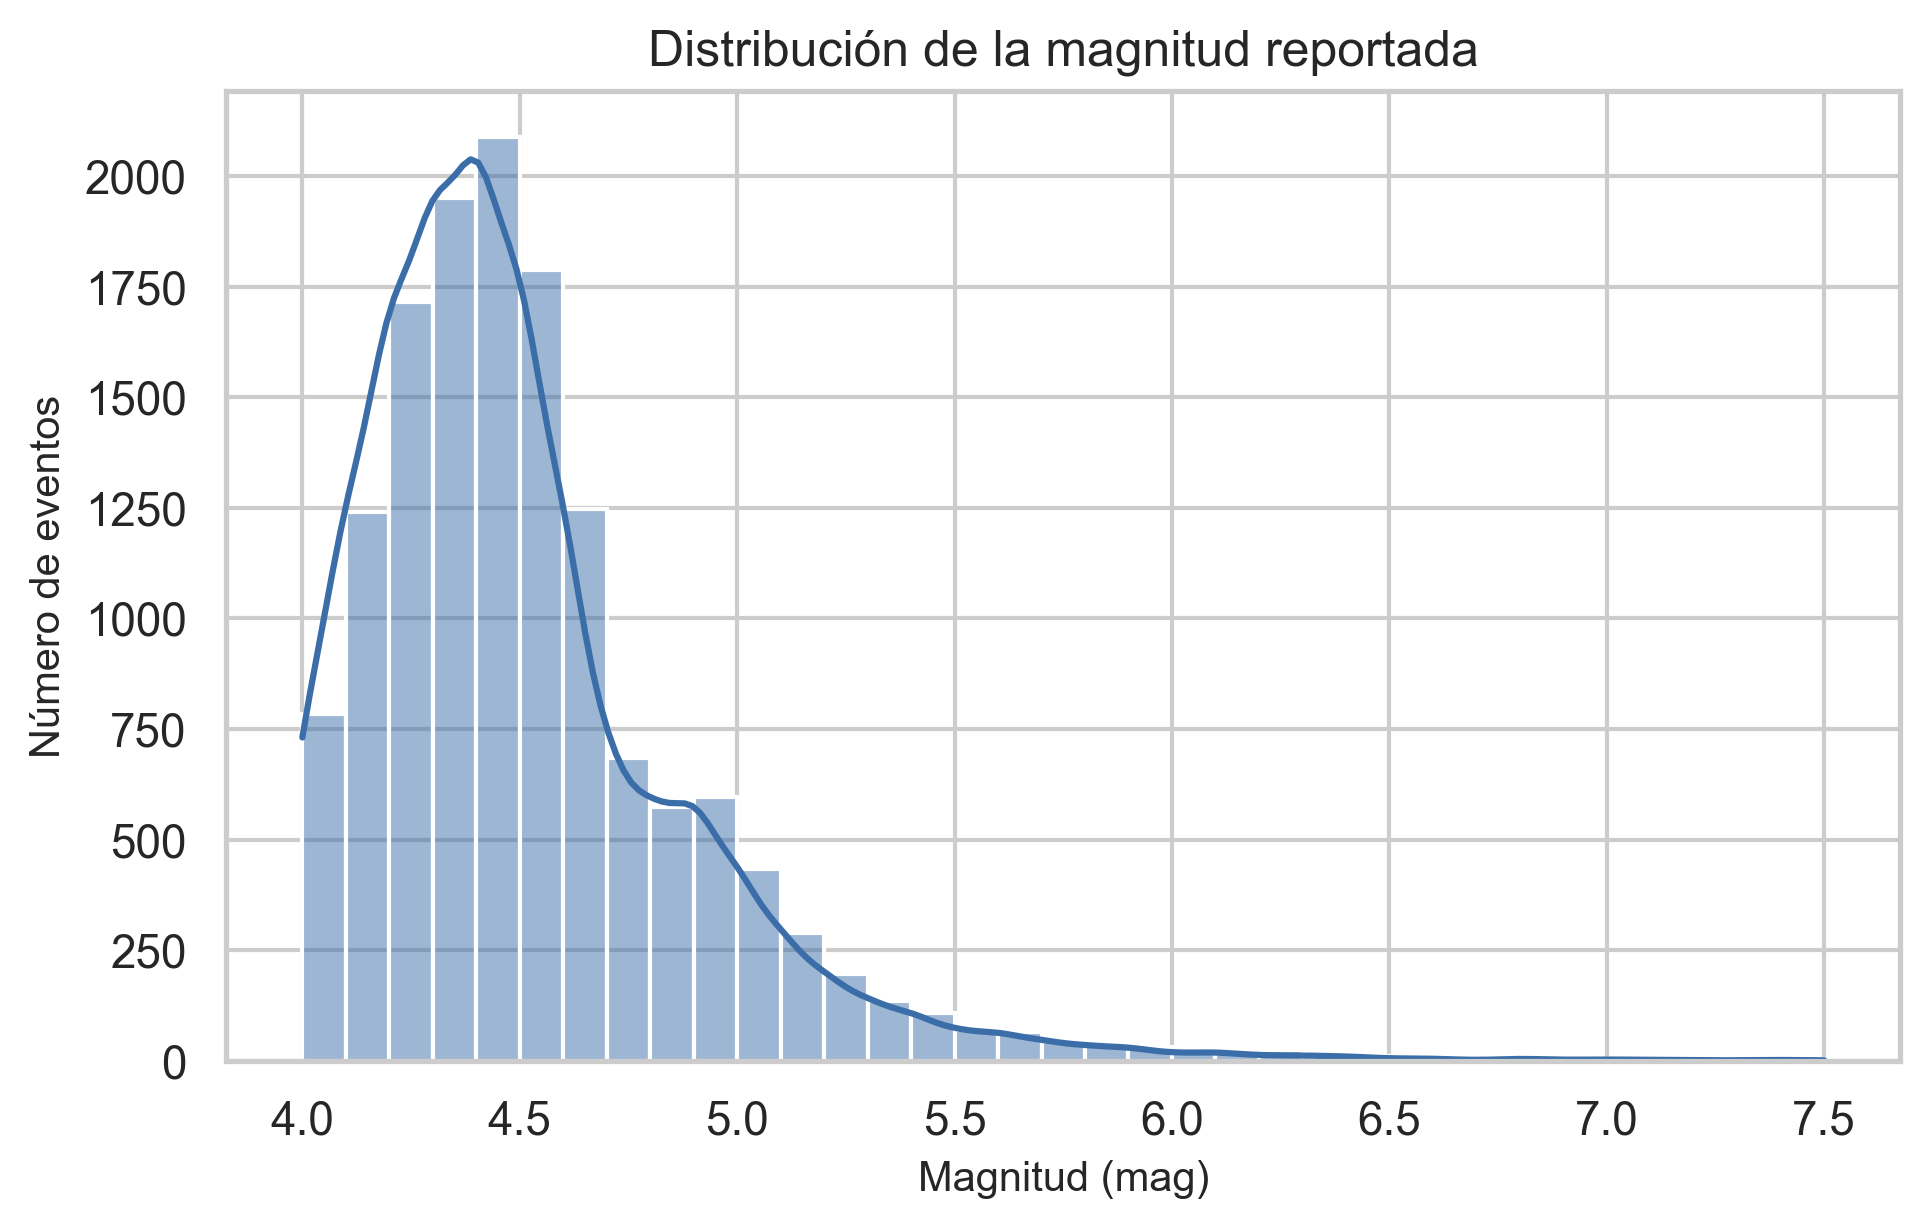
\includegraphics[width=\textwidth]{fig_hist_mag.png}
    \caption{Distribución de \var{mag}.}
\end{subfigure}
\hfill
\begin{subfigure}{0.48\textwidth}
    \centering
    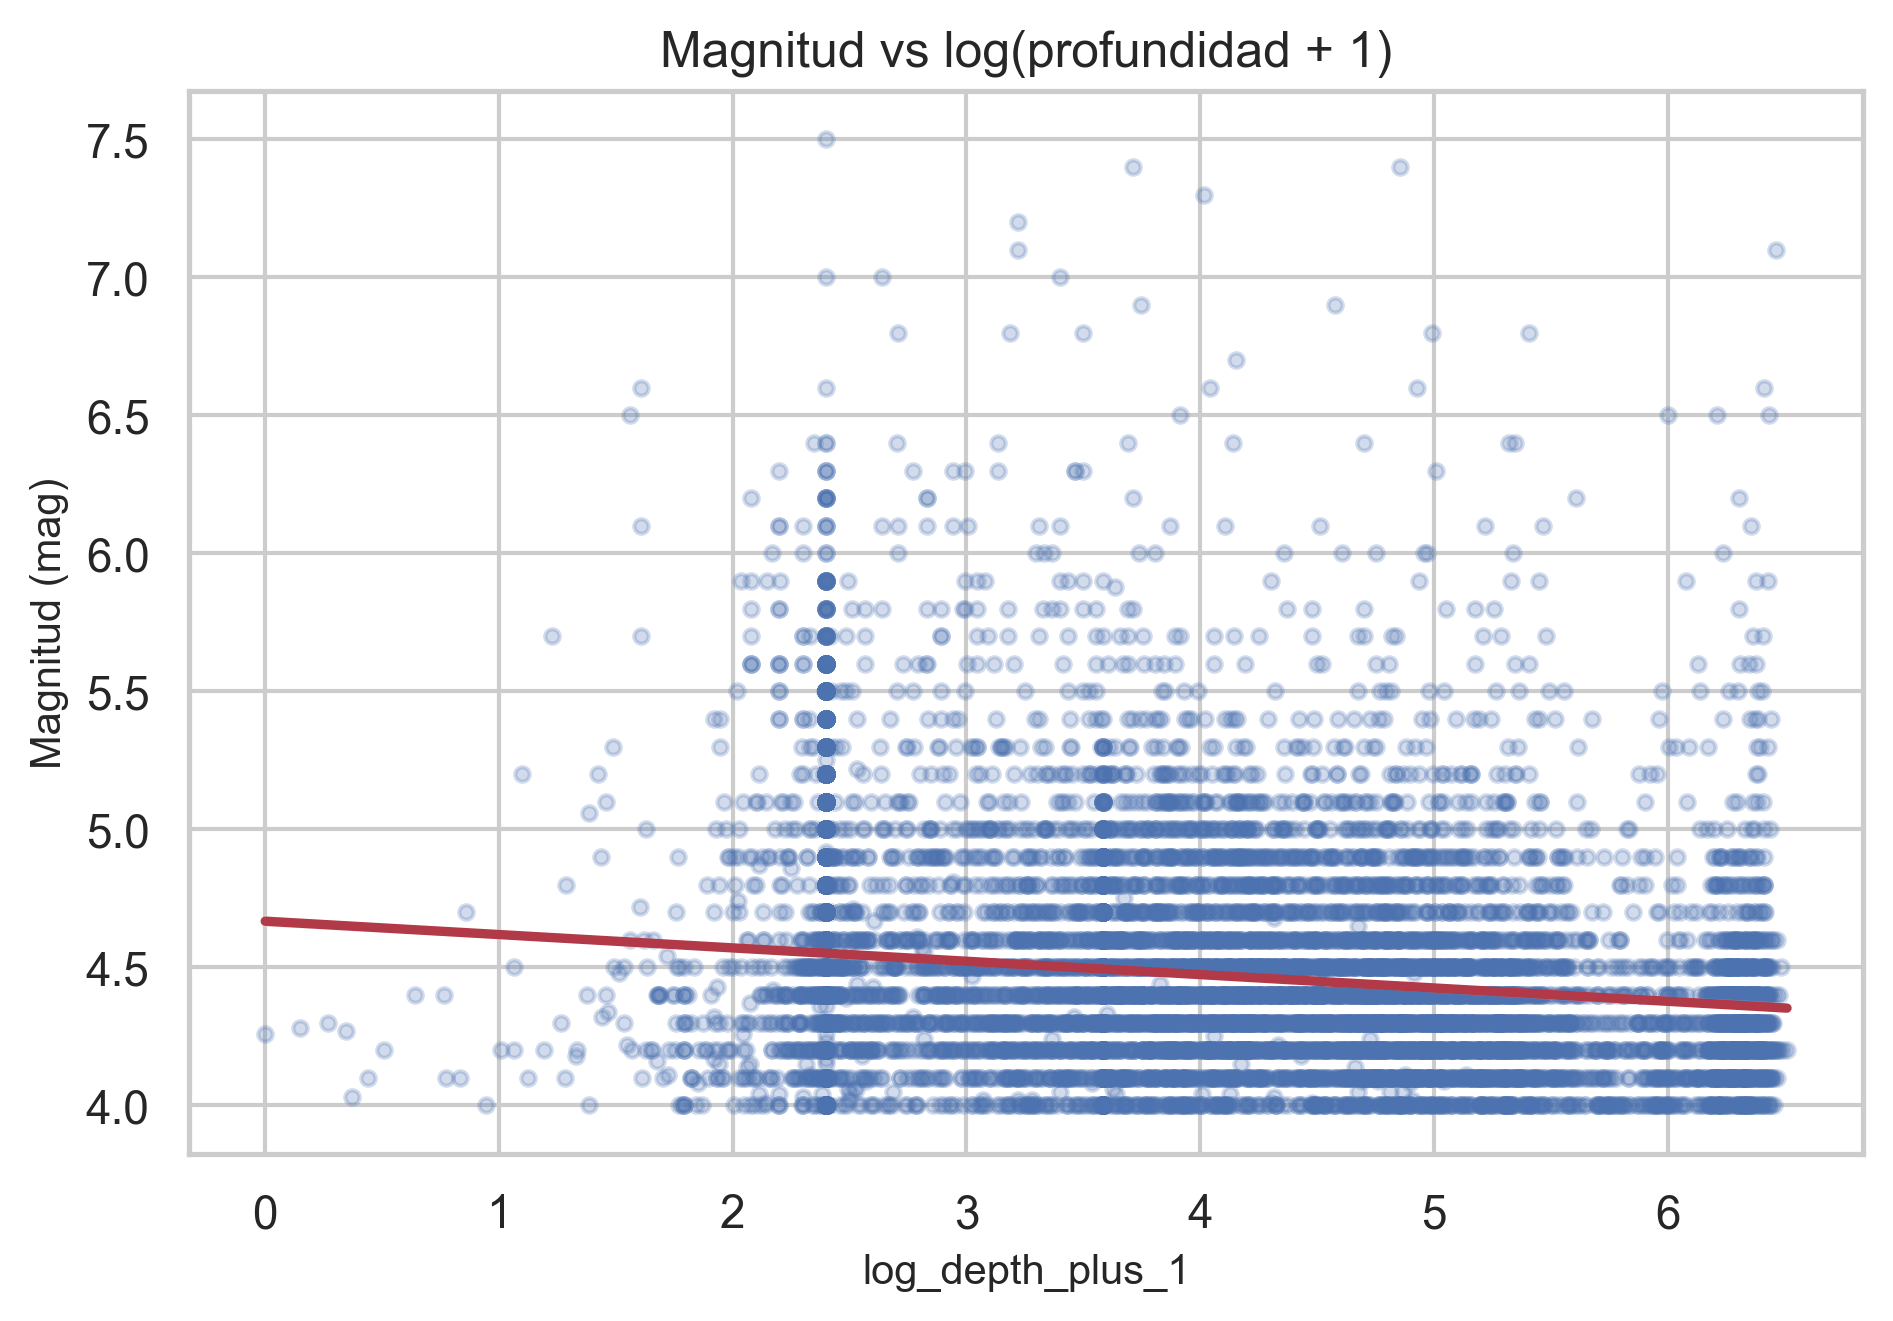
\includegraphics[width=\textwidth]{fig_scatter_mag_logdepth.png}
    \caption{\var{mag} y log profundidad.}
\end{subfigure}

\vspace{0.1cm}

\begin{subfigure}{0.48\textwidth}
    \centering
    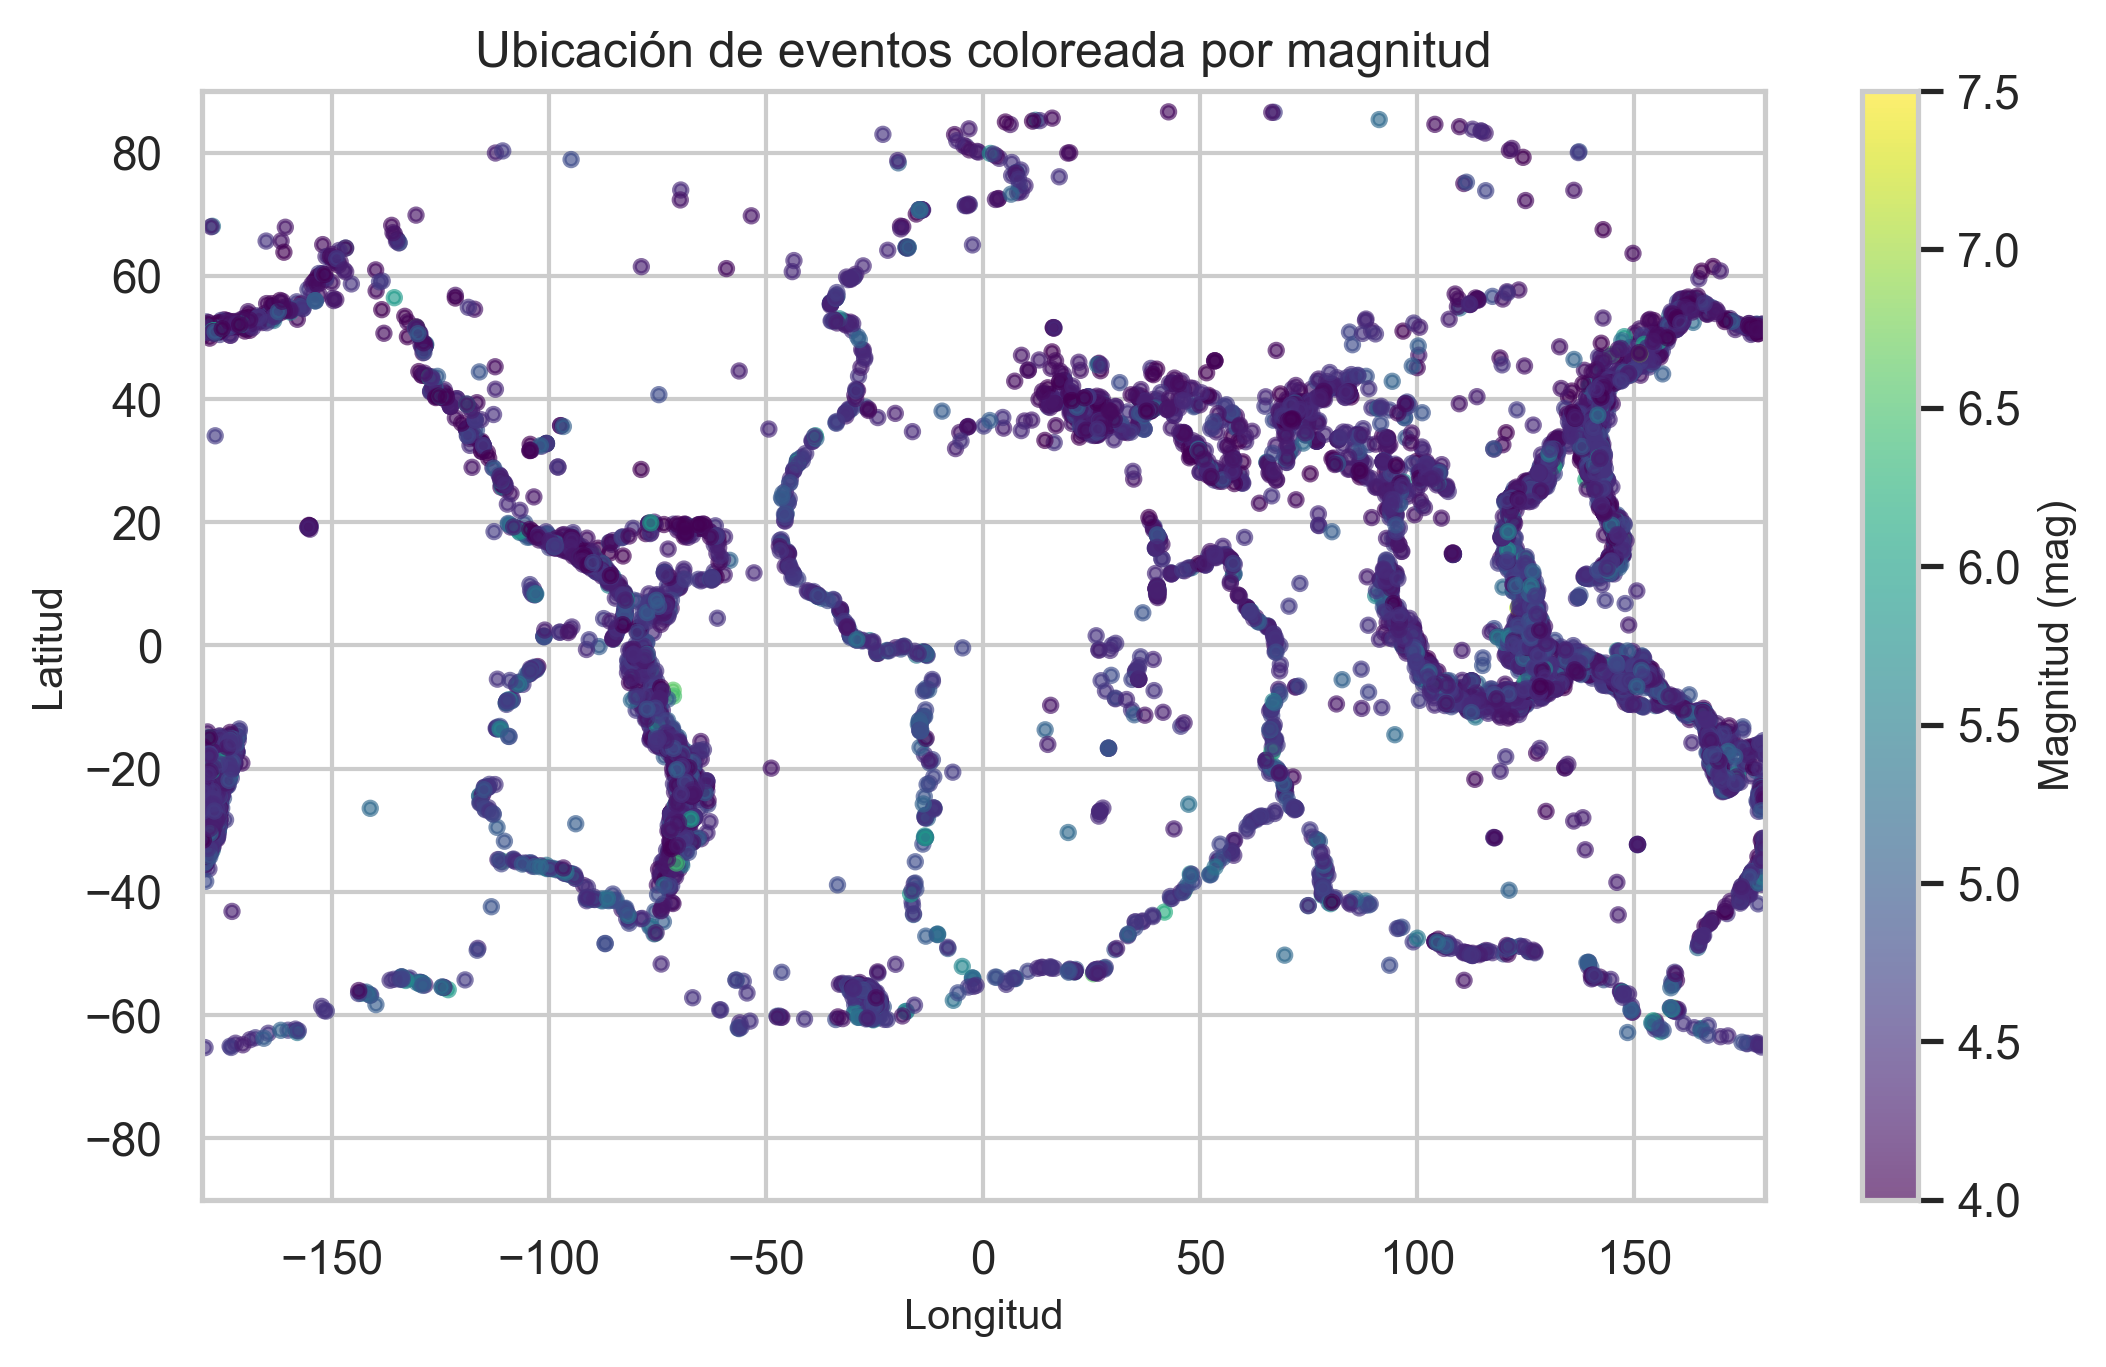
\includegraphics[width=\textwidth]{fig_map_mag.png}
    \caption{Ubicación coloreada por magnitud.}
\end{subfigure}
\hfill
\begin{subfigure}{0.48\textwidth}
    \centering
    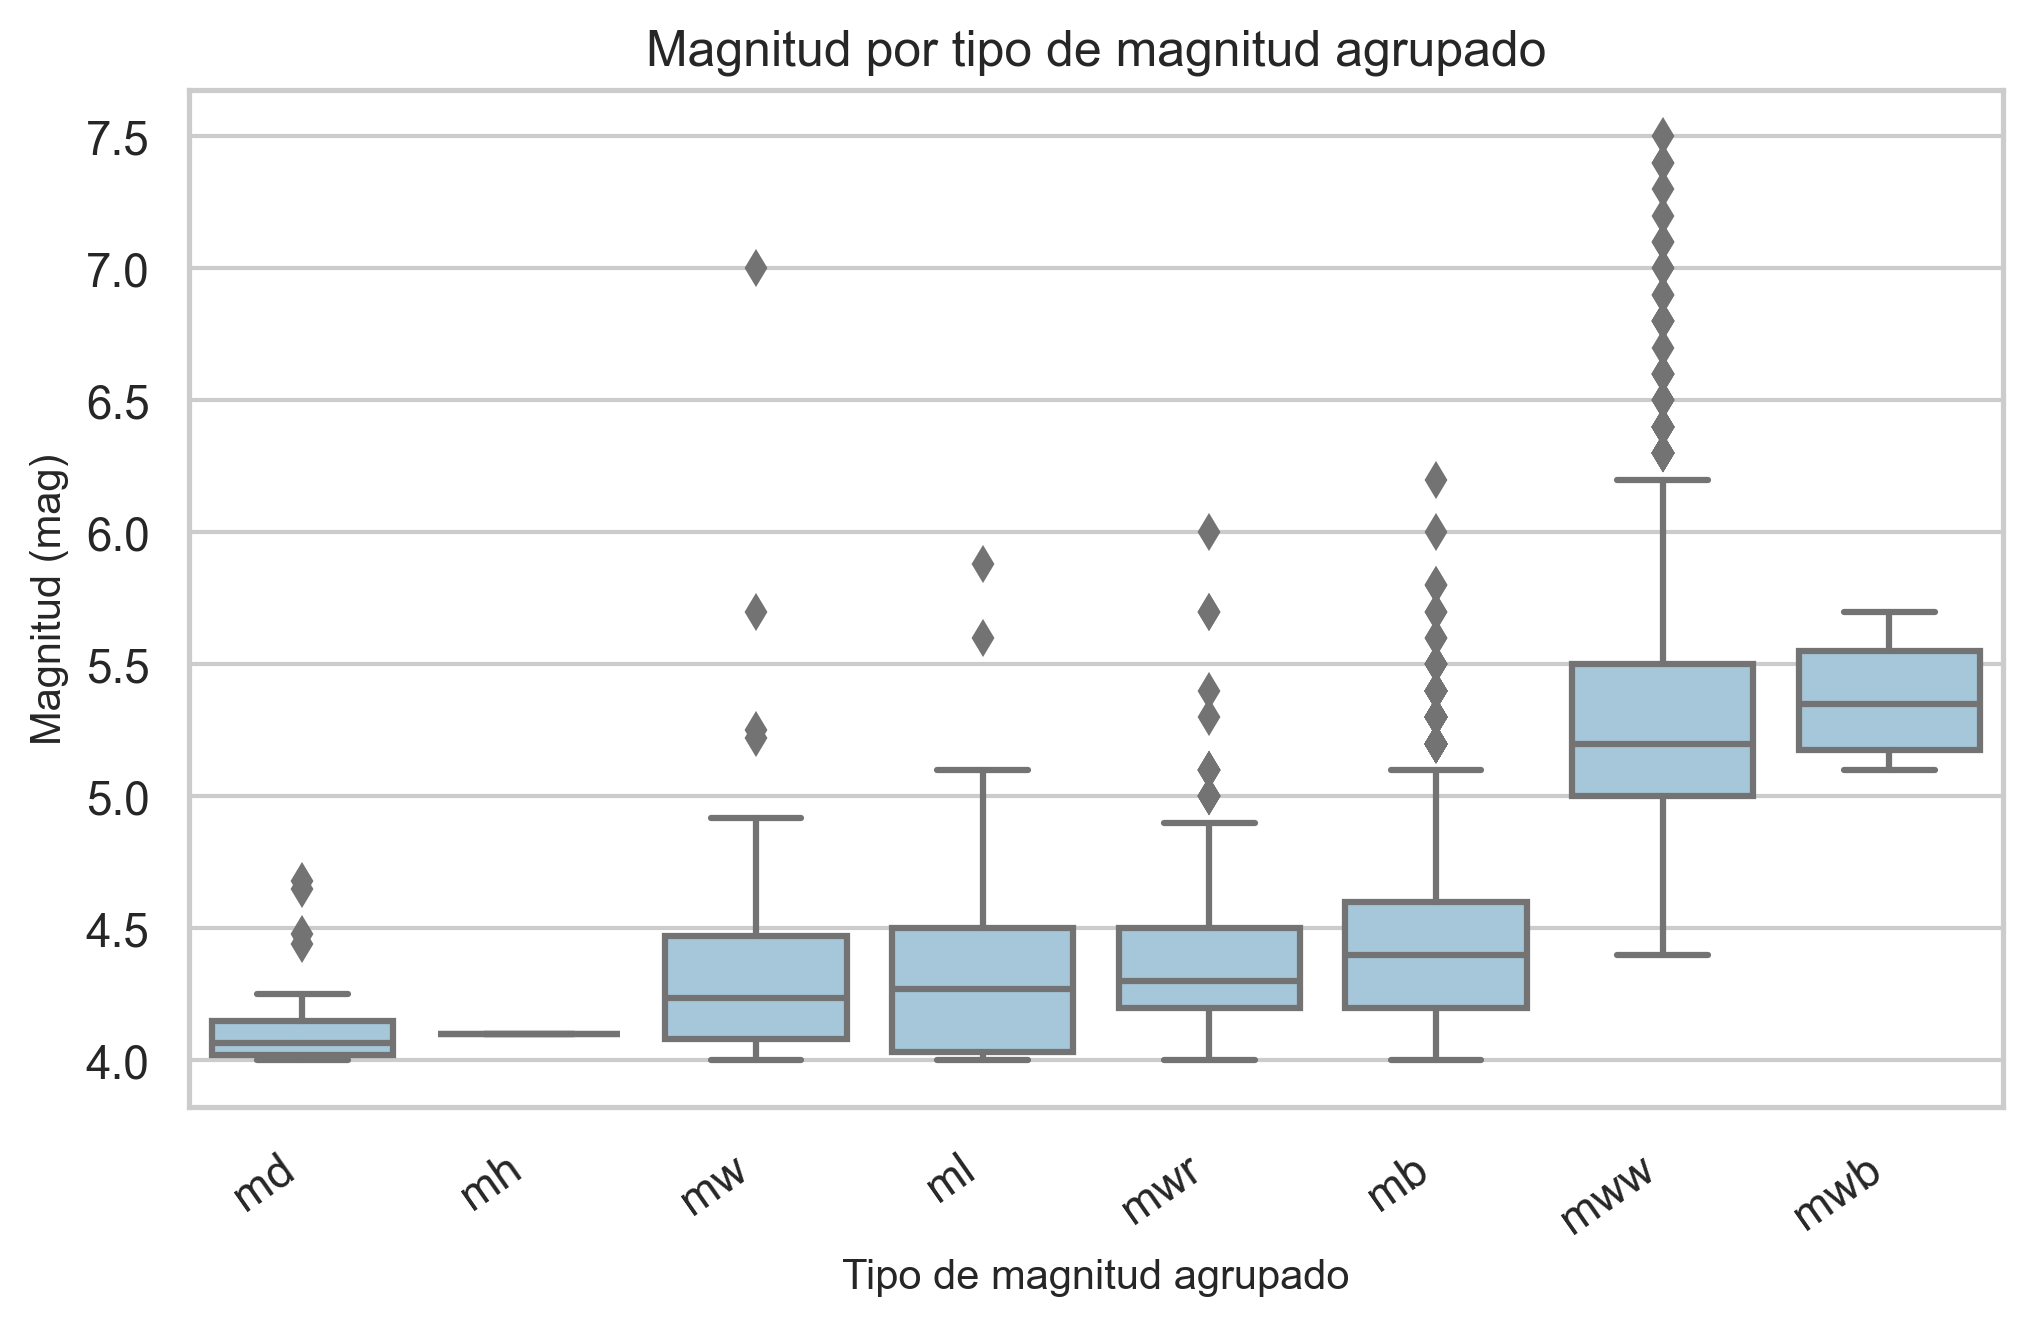
\includegraphics[width=\textwidth]{fig_box_mag_magtype.png}
    \caption{Magnitud por \var{magType}.}
\end{subfigure}
\vspace{0.12cm}
\caption{EDA principal ligado a la pregunta: distribución de la respuesta, asociación con profundidad transformada, patrón espacial y diferencias promedio por tipo de magnitud.}
\end{figure}

El EDA está directamente conectado con la pregunta de investigación. La magnitud aparece concentrada cerca del umbral 4 por el filtro de inclusión, por lo que las asociaciones se interpretan dentro de eventos moderados o mayores. El mapa muestra concentración espacial de eventos, lo que justifica incluir latitud y longitud como controles; además, las diferencias promedio por \var{magType} respaldan incorporar indicadores de tipo de magnitud. Estas relaciones son descriptivas y no se leen como efectos causales.

Las distribuciones de predictores complementan esta lectura: \var{log\_depth\_plus\_1}, \var{nst}, \var{gap}, \var{dmin} y \var{rms} muestran escalas y asimetrías distintas, lo que respalda revisar transformaciones y diagnósticos; las barras de \var{magType\_grouped} y \var{net\_grouped} muestran por qué conviene agrupar niveles poco frecuentes antes de usar indicadores.

%%%%%%%%%%%%%%%%% 4. PLAN DE MODELOS %%%%%%%%%%%%%%%%%
\section{Plan de modelos}

El avance considera una secuencia de modelos lineales interpretables. M1 evalúa la asociación marginal con profundidad transformada; M2 agrega ubicación básica mediante latitud y longitud; M3 incorpora variables técnicas del registro; M4 agrega diferencias promedio por tipo de magnitud; M5 revisa si la red de reporte captura diferencias adicionales; y M6 permite una relación espacial flexible con términos cuadráticos e interacción latitud-longitud, sin salir del marco de regresión lineal. Estas comparaciones evalúan qué bloque de variables aporta evidencia preliminar, controlando por las demás variables incluidas.

\begin{table}[H]
\centering
\caption{Bloques de modelos lineales candidatos}
\reporttablesize
\begin{tabularx}{\textwidth}{llX}
\toprule
Modelo & Bloque agregado & Propósito estadístico \\
\midrule
M1 & Profundidad transformada & Evaluar asociación marginal entre magnitud y profundidad. \\
M2 & Ubicación geográfica & Controlar por latitud y longitud del evento. \\
M3 & Variables técnicas & Incorporar cobertura y ajuste del registro sísmico. \\
M4 & Tipo de magnitud & Comparar diferencias promedio según método de magnitud. \\
M5 & Red de reporte & Evaluar diferencias adicionales asociadas a la institución reportante. \\
M6 & Términos espaciales flexibles & Permitir curvatura espacial mediante latitud, longitud, cuadrados e interacción. \\
\bottomrule
\end{tabularx}
\end{table}

{\reporttablesize
\begin{tabular}{lrrrrrrr}
\toprule
modelo & n & parámetros & R2 ajust. & AIC & BIC & RMSE & MAE \\
\midrule
M1 & 14176 & 2 & 0.028 & 12096.022 & 12111.141 & 0.371 & 0.268 \\
M2 & 14176 & 4 & 0.048 & 11801.695 & 11831.933 & 0.367 & 0.264 \\
M3 & 14124 & 8 & 0.535 & 1633.633 & 1694.079 & 0.256 & 0.184 \\
M4 & 14124 & 15 & 0.624 & -1361.202 & -1247.868 & 0.230 & 0.170 \\
M5 & 14124 & 22 & 0.625 & -1390.252 & -1224.028 & 0.230 & 0.170 \\
M6 & 14124 & 18 & 0.633 & -1688.352 & -1552.351 & 0.228 & 0.168 \\
\bottomrule
\end{tabular}

}

La comparación preliminar sugiere mejoras importantes al pasar de modelos puramente geográficos a modelos con variables técnicas y tipo de magnitud. Sin embargo, el modelo final no se escogerá solo por R2 o AIC/BIC: se priorizará interpretabilidad, diagnóstico de supuestos, colinealidad, observaciones influyentes y estabilidad ante categorías agrupadas. Dentro de esta etapa, M4 y M6 son candidatos naturales para diagnóstico inicial.

%%%%%%%%%%%%%%%%% 5. DIAGNÓSTICOS %%%%%%%%%%%%%%%%%
\section{Diagnósticos previstos y siguientes pasos}

En el informe final se revisarán residuos contra ajustados, normalidad aproximada mediante QQ-plot e histograma, heterocedasticidad potencial, distancia de Cook, leverage con residuos estudentizados y VIF para predictores numéricos principales. También se evaluará si quedan patrones espaciales en residuos. Dado que los datos son eventos puntuales, un modelo CAR no es el enfoque directo salvo que se agreguen observaciones por áreas o grillas; el foco del curso seguirá siendo regresión lineal múltiple, selección razonada de variables, inferencia y análisis de residuos.

Como análisis de sensibilidad se contrastarán decisiones razonables de transformación y especificación, por ejemplo usar \var{depth} versus \var{log\_depth\_plus\_1}, incluir o no variables técnicas con faltantes, y revisar la estabilidad de conclusiones ante observaciones influyentes. Esto permitirá distinguir patrones descriptivos robustos de resultados dependientes de una codificación particular.

%%%%%%%%%%%%%%%%% 6. REPRODUCIBILIDAD %%%%%%%%%%%%%%%%%
\section{Reproducibilidad}

El notebook \path{avance_proyecto_regresion.ipynb} genera la base procesada del proyecto (\path{usgs_earthquakes_2024_mag4_model_ready.csv}), las tablas en \path{Plantilla_informe/tables/} y las figuras en \path{Plantilla_informe/figures/}. El repositorio del proyecto está disponible en \url{https://github.com/Paul0112/proyecto_regresion}. Se documentan versiones de paquetes en \path{requirements.txt} y \path{session_info.txt}.

%%%%%%%%%%%%%%%%% REFERENCIAS %%%%%%%%%%%%%%%%%
\section*{Referencias}

\begin{enumerate}
    \item U.S. Geological Survey. \textit{Earthquake Catalog API}. Disponible en \url{https://earthquake.usgs.gov/fdsnws/event/1/}.
    \item Python Software Foundation. \textit{Python Language Reference}. Disponible en \url{https://www.python.org/}.
    \item Herramientas computacionales: se usó Python para limpieza, visualización y ajuste de modelos. Los resultados numéricos provienen de la ejecución reproducible del notebook sobre los datos locales.
    \item Declaración de uso de IA: se usaron herramientas de inteligencia artificial para mejorar el orden del informe, apoyar la generación de gráficos en Python y optimizar la disposición de imágenes en LaTeX.
\end{enumerate}

\end{document}
